
\documentclass[reqno,11pt]{book}
\usepackage{amsmath,amssymb,amsfonts} % Typical maths resource packages
\usepackage{graphicx}                 % Packages to allow inclusion of graphics
\usepackage{subfigure}                %to print pictures side by side
\usepackage{color}                    % For creating coloured text and background
\usepackage{hyperref}                 % For creating hyperlinks in cross references
%\usepackage[ddmmyyyy]{datetime}									
\usepackage[nodayofweek]{datetime}  	% To specify the date in UK form (instead of US)
 \usepackage{rotating}    %to allow large tables/pics to print on landscape
 \usepackage{setspace}

\def\cleardoublepage{\clearpage\if@twoside%              %To prevent empty pages apprearing before each chapter
  \ifodd\c@page\else\hbox{}\thispagestyle{empty}\newpage%
  \if@twocolumn\hbox{}\newpage\fi\fi\fi}

\parindent 1cm
\parskip 0.2cm
\topmargin 0.2cm
\oddsidemargin 1cm
\evensidemargin 0.5cm
\textwidth 15cm
\textheight 21cm
\newtheorem{theorem}{Theorem}[section]
\newtheorem{proposition}[theorem]{Proposition}
\newtheorem{corollary}[theorem]{Corollary}
\newtheorem{lemma}[theorem]{Lemma}
\newtheorem{remark}[theorem]{Remark}
\newtheorem{definition}[theorem]{Definition}


\def\R{\mathbb{ R}}
\def\S{\mathbb{ S}}
\def\I{\mathbb{ I}}
\makeindex


%TITLE PAGE

\makeatletter
\def\thickhrulefill{\leavevmode \leaders \hrule height 1pt\hfill \kern \z@}
\renewcommand{\maketitle}{\begin{titlepage}%
    \let\footnotesize\small
    \let\footnoterule\relax
    \parindent \z@
  \blurb
  \vspace{50mm}
    \begin{flushleft}
      \@title
    \end{flushleft}
    \par
    \hrule height 1pt
    \par
    \begin{flushright}
      \large \@author \par
    \end{flushright}
    \vspace{15mm}
     \begin{center}
    \normalfont
    {\normalsize \reqtexta\par}%
    \vskip 0cm
    {\normalsize \reqtextb\par}%
    \vskip 0.1cm
    {\Large \it \reqtextc\par}%
    \end{center}%
    \vspace{20mm}
    \begin{flushright}
    \arc
    \end{flushright}
     \vspace{15mm}
   \begin{flushright}
    \normalsize \@date
   \end{flushright}
    \vfil\null
  \end{titlepage}%
  \setcounter{footnote}{0}%
}
\makeatother


\def\blurb{%
  Department of Electrical \& Electronic Engineering \\
  The University of Melbourne\\ \\
  National ICT Australia (NICTA) }
\author{Elma O'Sullivan-Greene}
\title{\huge{The EEG As A Measurement Of Brain Activity: Towards Prediction of Epileptic Seizures}}
\date{\monthname, 2009}
\def\reqtexta{%
Submitted in total fulfilment of}
\def\reqtextb{%
the requirements of the degree of}
\def\reqtextc{%
Doctor of Philosophy}

% Comment out the following line for the copy submitted to the library
\def\arc {\ttfamily \small \fbox { {Produced on archival quality paper}}}



\begin{document}
\maketitle   %makes title page of document according to the commands in frontpage.txt
 
\chapter*{Abstract}\normalsize
  \addcontentsline{toc}{chapter}{Abstract}
  
\pagestyle{plain}
Abstract

The title page must be followed by:

    * An Abstract of 300-500 words in English. (In the case of creative arts the Abstract must include a description of the form and presentation of the creative work).
\pagebreak

\chapter*{Declaration}\normalsize
  \addcontentsline{toc}{chapter}{Declaration}
  
\pagestyle{plain}

This is to certify that

\begin{enumerate}
	\item The thesis comprises only my original work towards the PhD,
	\item due acknowledgement has been made in the text to all other material used,
	\item the thesis is less than 100,000 words in length, exclusive of tables, maps, bibliographies and appendices.
\end{enumerate}



\vfill

\hspace*{\fill}
\begin{minipage}{4in}
\flushright
~\hrulefill\vskip 1ex
~{\bf Signature}\vskip 7ex
~\hrulefill\vskip 1ex
~Date
\end{minipage}

\vfill


\pagebreak

\chapter*{Acknowledgements}\normalsize
  \addcontentsline{toc}{chapter}{Acknowledgements}
  
\pagestyle{plain}
\input{acknowledgements}
\pagebreak

\addcontentsline{toc}{chapter}{Contents}
\pagenumbering{roman}
\pagestyle{headings}
\tableofcontents
\listoffigures
 \addcontentsline{toc}{section}{List of Figures}
\listoftables
 \addcontentsline{toc}{section}{List of Tables}
\include{abbreviations}



%\chapter*{Preface}\normalsize
%  \addcontentsline{toc}{chapter}{Preface}
  
%\pagestyle{plain}
%The text for preface


\chapter*{Introduction}\normalsize
  \addcontentsline{toc}{chapter}{Introduction}
  
\pagestyle{plain}
\onehalfspacing

\label{ch:intro}

Introduction section text...

\pagebreak
\pagestyle{headings}
\pagenumbering{arabic}


\numberwithin{table}{section}   %otherwise table will be labeled "Table 1.1", but when referenceing withing the text will get "see Table 1.3.1"
%may later have to do the same with equations
\numberwithin{equation}{section}

%other examples
%\numberwithin{equation}{section}
%\numberwithin{figure}{section}
%\numberwithin{table}{section}
%\numberwithin{equation}{chapter}
%\numberwithin{figure}{chapter}
%\numberwithin{table}{chapter}

%% ch1.tex
\chapter{Neurophysiology Background}
\label{ch:neurobackgnd} 
%%%%%%%%%%%%%%%%%%%%%%%%%%%%%%%%%%%%%%%%%%%%%%%%

% 1111111111111111111111111111111111111111111111111111111111111111111111111111

\section{Structure of the Brain}
\label{sec:struct}

The brain together with the spinal cord make up the central nervous system, the body's sensory analysis and decision making system. \cite{Kandel_2002_PrinciplesNeuralSc,Sherwood_2001_cell2sys,Nunez_2006_ElecFieldsBrain} provide the following information regarding the anatomy of the brain. The brain can be subdivided into two main regions, the brainstem and cerebrum. The cerebrum is structurally divided into two main regions each called a cerebral hemisphere.  The outer layer of the hemispheres is known as the cerebral cortex. The cortex is a much folded structure which is estimated to contain in the order of $10^{10}$ nerve cells or $\it{neurons}$ \cite[Ch. 1]{Nunez_2006_ElecFieldsBrain}.  The cortex contains both ``grey matter'' and ``white matter''.  Grey matter is a layer containing a high density of neuron cell bodies while, the white matter, located underneath the grey matter, is largely composed of  nerve  fibers or $\it{axons}$.  The cortex is further divided into four main lobes, each with its own function specification, see Figure~\ref{fig:brainsurf}.  The brain stem connects the spinal cord to the cerebral cortex, via the thalamus, a deep brain structure which gates the information flow from the brainstem to the cortex, see Figure~\ref{fig:brainmid}.\\

\begin{figure} [hbt]
\centering
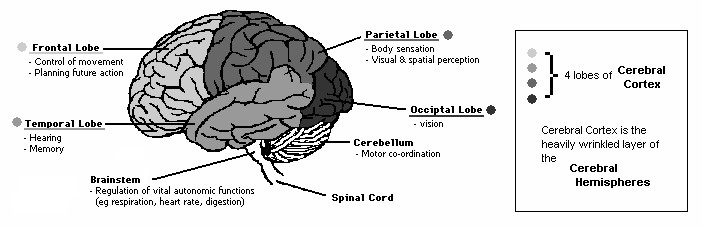
\includegraphics[height=2.1in]{figures/070108_brain_parts}
\caption{Surface view of the brain, illustrating the main lobes of the cerebral cortex and their basic functions, taken in part from \cite{corteximage} }
\label{fig:brainsurf}
\end{figure}

\section{Epilepsy}
\label{sec:epilepsy}

The International League Against Epilepsy (ILAE) defines an epileptic event as ``a transient occurrence of signs and symptoms due to abnormally excessive or synchronous neuronal activity in the brain''\cite{Fisher_2005_DefinitionsfromILAE}.  Epilepsy is defined as ``a disorder of the brain characterised by an enduring predisposition to generate epileptic seizures''\cite{Fisher_2005_DefinitionsfromILAE}, and is usually not diagnosed until more than one epileptic event has occurred.\\     



\section{Electroencephalography}
\label{sec:eeg}

Electroencephalography (EEG) is a record of the temporal fluctuations of electrical potentials recorded from electrodes on the human brain. \\


\subsection{Interpretation of the EEG}

subsection text.....
%% ch2.tex
\chapter{Literary  Review}
\label{ch:review} 
%%%%%%%%%%%%%%%%%%%%%%%%%%%%%%%%%%%%%%%%%%%%%%%%


chapter 2 text
%%  ch3.tex
\chapter{Name of Chapter 3}
\label{ch:3} 
%%%%%%%%%%%%%%%%%%%%%%%%%%%%%%%%%%%%%%%%%%%%%%%%

text of chapter 3 ...








 \bibliography{Bib_thesis}
  \addcontentsline{toc}{chapter}{Bibliography}

   \bibliographystyle{unsrt}

  %\addcontentsline{toc}{chapter}{Index}

\end{document}